\documentclass[doktyp=parbeit, hausschrift=false, sprache=english, fontsize=12pt]{TUBAFarbeiten}

\usepackage{amssymb}
\usepackage[fleqn]{amsmath}
\usepackage{MnSymbol}
\usepackage{enumitem}
\usepackage[geometry]{ifsym}
\usepackage{csquotes}
\usepackage{cite}
%\usepackage{graphicx}
%\usepackage{stackengine}
\usepackage{pgfplots}
\usepackage{bbm}
\usepackage[english]{babel}
\usepackage{hyperref}
\usepackage[english]{cleveref}

\TUBAFTitel{Monocular Depth Estimation on Artificially Scaled Up Camera Images for Robot Applications}
\TUBAFAutor{Nico Zumpe, Johannes Kohl}
\TUBAFMatrikel{62\,351, 64\,751}
\TUBAFDatum{14.08.2023}
\TUBAFBetreuer{Dr. Sandra Lorenz}
\TUBAFStudiengang{Robotik (Diplom)}
\TUBAFFakultaet{Fakultät für Mathematik und Informatik}
\TUBAFInstitut{Institut für Informatik}

\graphicspath{{../resources}}

\usetikzlibrary{math}
%\usetikzlibrary{positioning}
\usetikzlibrary{decorations.pathreplacing,calligraphy}

\linespread{1.25}

\pgfplotsset{compat=1.16}
\begin{document}

\maketitle

\begin{abstract}
    In the field of robotics it is still somewhat of a challenge to analyse objects and scenes in camera images that are far away from the robot.
This might not be problematic for many stationary and/or slow moving platforms, but it is easy so see what issues may arise when the speed increases or timing in general gets critical.

Combating this problem can be done by, for example, changing the lens of the camera, which in turn hurts the field of view (FOV). \\
Another approach would be to employ a higher resolution camera. The problem here is that more bandwidth, aswell as higher computing power would be needed to transport and process those images.
So every advance into more depth clarity comes with it's own tradeoffs.

Therefor a solution with a smaller cost is needed. For this goal, the \enquote{higher resolution} approach may still be a viable option by using AI upscaling.
The idea is to use a supersampling model to \enquote{enhance} certain regions of interest in the source image and analyse them further.
For the sake of evaluation this further analysis will be performed as monocular depth estimation.

%TODO: add results
\end{abstract}
\section{Introduction}
\section*{Introduction}

A person operating a motor vehicle always needs to be aware of their surroundings and the environment. They know that the car they saw coming on the background is not gone because the turning car in front of them is blocking it.  This phenomena is called object permanency and is something the majority of humans learn growning up.
That same concept is not hard for a computer to grasp either but what might be is the preamble of \enquote{detecting the car in the background}. Robots rely heavily on images to orient themselves in their environments but this brings some limitations.
There are some options to combat this, but they either come with their own tradeoffs or may not be aplicable in all situations.

Changing to a camera with a thicker lense will improve the zoom, but since the image size stayed the same the overall field of view (FOV) is decreased. This may affect close by detection and analysis.
As a fix for the above method or a standalone approach it might be useful to change recording resolution to something greater. But also this approach has drawbacks as it required way more bandwith and computing power to process those larger images.
Another fix to the lens problem might be varifocal lenses but they add in complexity/cost and might not be easily applicable in stereo camera setups since both lenses would need to be well synchronized.

A comparatively low cost solution arises in image superresolution implemented as an AI supersampling model. With this method no extra hardware equipment would be needed.
There would still be an overhead though, but it can be held down by only supersampling specific regions of interest like the end of a road, intersections, entrances, etc.

\section{Background}
Since we merge and use two aspects of image processing in this project, image super-resolution and depth estimation, we also highlight both aspects separately.
The merging process will be explained later in the implementation chapter.
\subsection*{Super Resolution}

Super-Resolution is an active research topic, which focuses on recovering a high-resolution image from a low-resolution image. In the paper we used, the main goal is to achieve better overall perceptual quality for super-resolution. In this paper used for our algorithm the basic architecture of SRResNet is used. \cite{wang2018esrgan}

\begin{figure}[ht]
    \begin{center}
        \includegraphics*[scale=.4, pagebox=artbox]{resources/Background_SR_1.png}
        \caption{ESRGAN architecture. \cite{wang2018esrgan}} \label{ESRGAN_arch}
    \end{center}
\end{figure}

To improve the quality of the recovered image by the super-resolution, there are 2 modifications made to the structure of the generator. Firstly all Batch Normalization layers are removed. Secondly the replacement of the original basic blocks with the Residual-in-Residual Dense Blocks (RRDB). Those combine multi-level residual networks and dense connections.

\begin{figure}[ht]
    \begin{center}
        \includegraphics*[scale=.4, pagebox=artbox]{resources/Background_SR_2.png}
        \caption{Improvements to the architecture. \cite{wang2018esrgan}} \label{rESRGAN_nw}
    \end{center}
\end{figure}

The discriminator based on the Relativistic GAN is also enhanced. The relativistic discriminator tries to predict the probability that a real image is relatively more realistic than a fake one. Specifically in[Ref paper] they replaced the standard discriminator with the relativistic average Discriminator RaD.

Also a more effective perceptual loss is developed. Perceptual loss is defined on the activation layers of a pre-trained deep network. In that Network the distance between two activated features is minimized. It is changed so the features are used before the activation layers. A more suitable perceptual loss is developed based on a fine-tuned VGG network for material recognition. It focuses more on textures rather than objects, because the researcher in [Referenz Paper] believe that perceptual loss focused on texture ist critical for super-resolution.

Because there is undesired noise in GAN-based methods, a flexible and effective strategy is proposed which is called network interpolation. First a PSNR-oriented network is trained and out of that a GAN-based network is obtained due to fine-tuning. All corresponding parameters of the two networks are interpolated to get an interpolated model. This interpolated model has two advantages. First it is able to produce meaningful results for any usable interpolation parameter without introducing artifacts. Secondly it's possible to continuously balance perceptual quality without the need of re-training the model.




\subsection*{Monocular Depth Estimation}

Depth sensing is traditionally done utilizing multiple lenses with a fixed and known distance and orientation. This concept is based on observations of nature and is also the way our eyes work.
But apart from this, there are not many methods of "spatial vision". One of those other methods is monocular depth estimation where a depth image is to be guessed from a single perspective by a neural network. Initial works in this area of research are for example 
%[Saxena et al., 2008; Eigen et al., 2014; Huynh et al., 2020; Yin et al., 2019]
. There attempts were made to utilize Markov random fields and simpler versons of current concepts like DNN feature encoding.
Through time many implementations and methods for optiomization where developed. Reletive recently 
%[Kim et al., 2022]
proposed Global-Local Path Networks consisting of an encoder and decoder following a global path with skip connections running into "Selective Feature Fusion" (SFF) modules for local features. The general structure can be seen in figure \ref*{GLPDepth_arch}.

\begin{figure}[ht]
    \begin{center}
        \includegraphics*[scale=.22, pagebox=artbox]{resources/GLPDepth.png}
        \caption{GLPDepth architecture} \label{GLPDepth_arch}
    \end{center}
\end{figure}

The Encoder consists of 4 (encoding) feature stages with an encoding block each. Between stages the dimensions get reduced by scales $\frac{1}{4}$, $\frac{1}{8}$, $\frac{1}{16}$, $\frac{1}{32}$. This in done to reduce computational overhead. The first 3 stages also host skip connections into the decoder wich will be talked about later.

The Decoder itself follows a similar but reversed structure as the encoder. It scales the dimensions back up by $\frac{1}{16}$, $\frac{1}{8}$, $\frac{1}{4}$ and $\frac{1}{2}$. Inbetween those upsampling steps are so called SFF modules wich merge global features with local features from the skip connections. Their specific construction is as depicted in figure \ref*{SFF_arch}.

\begin{figure}[ht]
    \begin{center}
        \includegraphics*[scale=.2, pagebox=artbox]{resources/SFF.png}
        \caption{SFF architecture} \label{SFF_arch}
    \end{center}
\end{figure}

According to the researchers, a big performance boost for GLPDepth was also a data augmentation method they called Vertical CutDepth. It is an offspring of the CutDepth method
%[Ishii and Yamashita, 2021]
which cuts a region of interest (ROI) from the source image to create a "new" datapoint. The difference with Vertical CutDepth is, that the ROI only takes a random horizontal position and width but always remains at $y=0$ with the full height. This is due to findings 
%[Dijk and Croon, 2019]
in previous depth estimation networks which suggest that they focus more on veritcal then horizontal features.
\section{Implementation}
\subsection{Peak Signal Noise Ratio}

The signal to noise ratio is a common tool to get a measurement of how much a signal is influenced by random noise. It is calculated by weighing the power of the signal itself against the power of the noise.
\begin{align}
    SNR = \frac{P_{\text{Signal}}}{P_{\text{Noise}}}
\end{align}
As images can be seen as discrete signals in two dimensions this concept can also be applied. To avoid evaluating every pixel individually the peak signal to noise ratio (PSNR) can be used which represents the maximum over the signal to noise ratio. In order to calculate it the mean squared error (MSE) over the difference between the image in question and the original image is needed. Typically the PSNR is calculated logarithmically to accommodate a wide range of MSEs.
\begin{align}
    PSNR &= 10 * \log_{10}(\frac{R^2}{MSE}) [\mathrm{dB}] \\
    \text{with: } & R = 255 \text{ …maximum fluctuation in the input image data type} \nonumber \\
    & MSE \text{ …mean squared error} \nonumber
\end{align}
As a general rule of thumb a higher PSNR means a better result and a better quality image.
A note for this implementation: When the MSE equates to zero $-1$ is returned as the PSNR would be $\infty$ which would make further calculations difficult.


\subsection{Monocular Depth Estimation} \label{mde_impl}

To lay a baseline for the accuracy of the GLPDepth model we compared it to a ground truth and calculated the MSE, PSNR in Dezibel and computation time. To do this we utilized svo files generated by a Stereolabs ZED2i stereo camera. Those files contain the video streams of both lenses, as well as of all other sensors. In our case the videostream had a resolution of 1920x1080 and was recorded with a framerate of 15fps.
The accompanying ZED SDK was used to calculate the depth images from that stereo camera setup as the ground truth. As will be discussed later, this is not necessarily optimal but sufficient.
The logged data gets temporarily stored in a numpy array and later written to an output csv file along with the frame index and time. The median and mean values over the aforementioned critical values get calculated in post, just before saving.


\subsection{super-resolution}

The implementation is kept simple. First the given raw-images get scaled down by $4$ using the resize method of OpenCV.

\begin{figure}[ht!]
    \begin{center}
        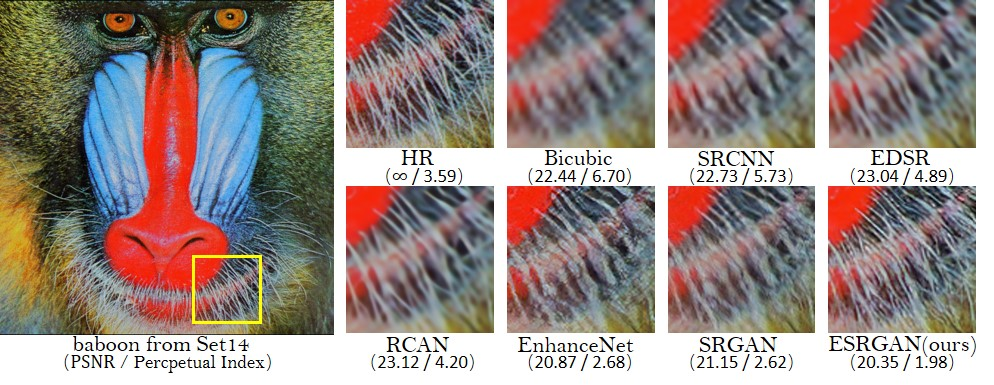
\includegraphics[scale=.44]{resources/qualitative_cmp_01.jpg}
        \caption{Comparison of the used super-resolution image to other models. \cite{ape_bib}} \label{ape}
    \end{center}
\end{figure}

Then the pretrained model gets loaded which can be obtained in the README of the ESRGAN \href{https://github.com/xinntao/ESRGAN}{repository} and yields results as shown in figure \ref*{ape}. As can be seen it compares quite well against other super-resolution models. In the repository are two models ready to use, the RRDB\textunderscore ESRGAN\textunderscore x4.pth and the RRDB\textunderscore PSNR\textunderscore x4.pth. We tested them both and stayed with the ESRGAN model. After loading the model with the parameters, the low resolution images get applied.

Lastly the PSNR is calculated over the raw images and the results after the process.

\subsection{Combination}

\begin{figure}[ht!]
    \begin{center}
        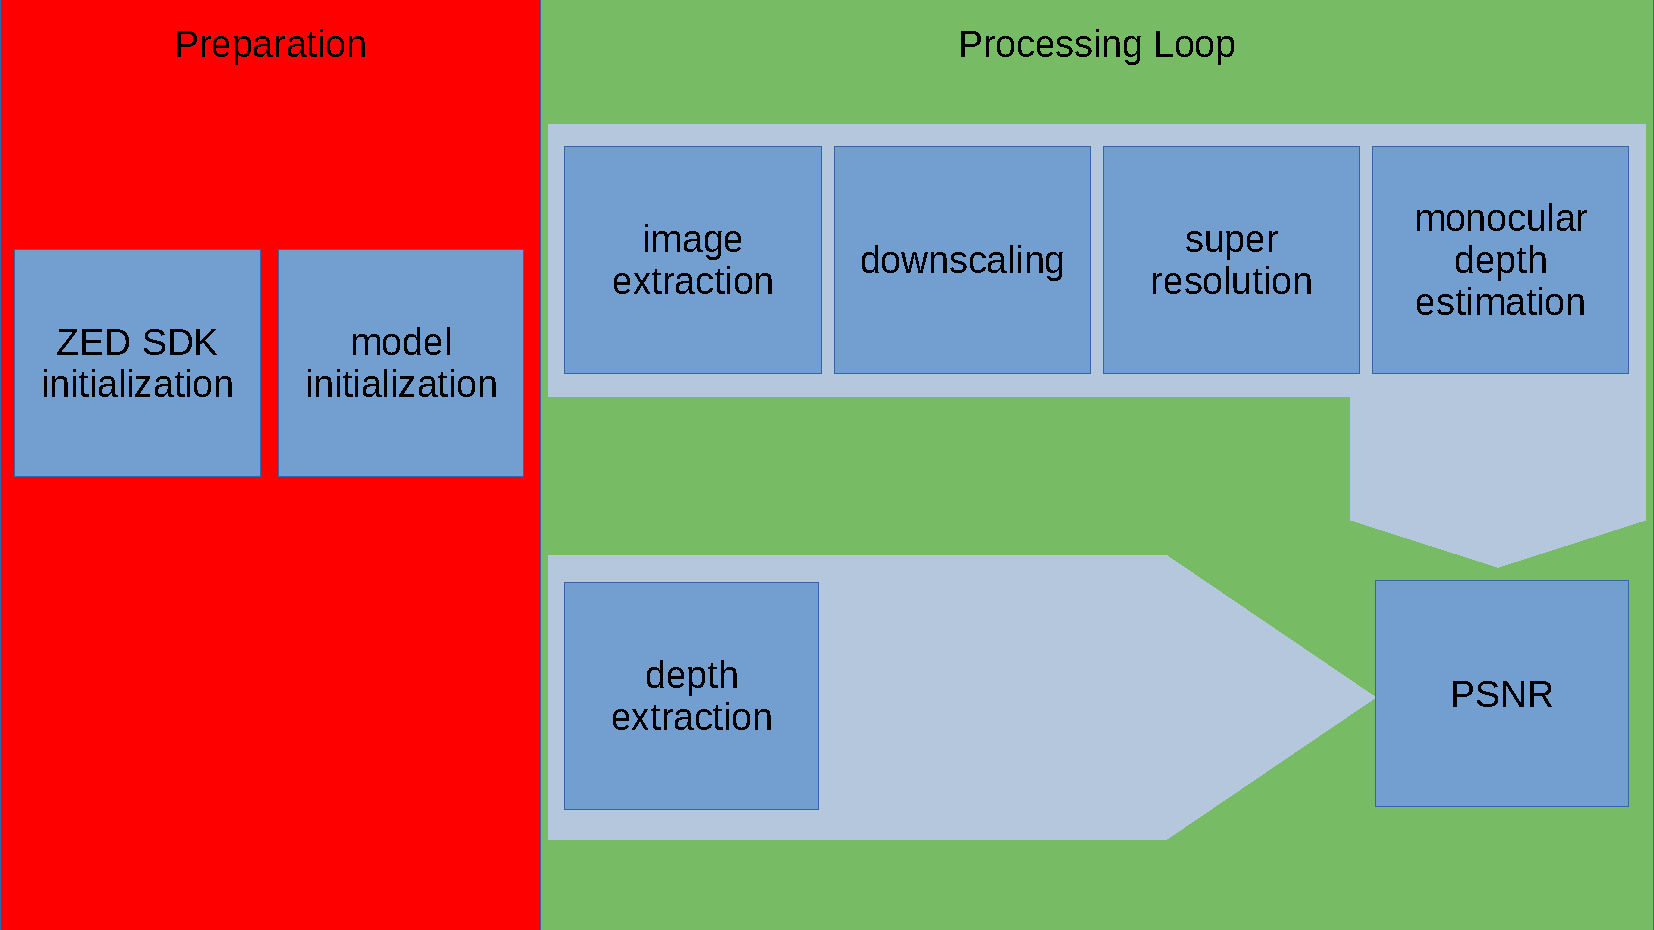
\includegraphics[scale=.5]{resources/general_plan.pdf}
        \caption{Flowchart of the final implementation.} \label{flowchart_general}
    \end{center}
\end{figure}

The actual implementation is very similar to the baseline implementation (Chapter \ref*{mde_impl}) in that there is a ground truth extracted from the given stereo information. But since the fine-grained information which would be the goal of the extraction with the super-resolution is not available via this method the effect is approximated by first downscaling the left camera image by a factor of $4$ using OpenCV and subsequent upscaling via the super-resolution model. This upscaled image is then used as an input for the monocular depth estimation model to produce a depth image which in turn is compared against the ground truth. Again MSE and PSNR are used to determine the quality of the generated prediction. The time it took to process the images in the neural networks is also logged. Those evaluations are then stored and later saved to a csv file along with the mean and median values of the processing time, MSE and PSNR for evaluation.

The max depth is taken from the parameters used for the svo recording, which in this case is a range from $0.3\mathrm{m}$ to $20.0\mathrm{m}$. The initialization values for the GLPDepth model are taken from the original implementations  \href{https://github.com/vinvino02/GLPDepth}{repository} to accommodate the respective pretrained weights. The latter can also be downloaded as stated in the repositories README. Only nyudepthv2\textunderscore swin\textunderscore large.ckpt and kitti\textunderscore swin\textunderscore large.ckpt are needed.

The two pretrained weights available to choose from differentiate in the dataset used for training. One was trained on the KITTI Eigen Split while the other one was trained on Nyu Depth V2. These datasets are different from each other in the sense that the former covers primarily the outdoors while the latter contains inside references.

All images are cut or resized to a size of 1216x352 which is rather arbitrary and thus just adopted from the original implementation. This size could be some other size that fulfills the rule of being divisible by 4 without a remainder in both directions. This constraint is necessary since the code does not explicitly check for mismatches between the ground truths size and the resulting depth estimations size resulting from a potential violation of this rule.
\section{Experimental Evaluation}
\subsection{Monocular Depth Estimation}

\begin{table}[ht!]
    \begin{center}
        \begin{tabular}{ l | r r r r }
                                & \multicolumn{2}{c}{Nyu Depth V2}  & \multicolumn{2}{c}{KITTI} \\
                                & cropped   & resized               & cropped   & resized       \\
            \hline
            execution time [s]  & 0.524     & 0.528                 & 0.299     & 0.306         \\
            MSE                 & 10.334    & 30.742                & 1.761     & 0.478         \\
            PSNR [dB]           & 38.001    & 33.258                & 45.864    & 51.761        \\
        \end{tabular}
        \caption{Results of GLPDepth alone. Mean and median did not differ much, so only the mean is depicted.} \label{res_glpdepth}
    \end{center}
\end{table}

One preparation step was to lay a baseline of how good the depth estimation performs in real world robotics applications. To do this the same pipeline was used as for the final algorithm (See chapter \ref*{general_subsection}) except for the downscaling and super-resolution steps in between. By doing this it is possible to get a perspective on a possible negative impact from the super-resolution. It also makes it possible to roughly estimate this impact. Furthermore it enables comparisons against conventional methods and discussions about the practicability and useability of this application. The results are displayed in figure \ref*{res_glpdepth}.

In the data various trends are visible. Firstly it is apparent that KITTI seems to perform better across the line on our data which checks out with the closeness to the automotive sector that robotics has. Secondly it seems that preserving the whole image by scaling it down instead of cropping it helps the algorithm to make better predictions. This is undoubtedly related to findings in the context of Vertical CutDepth \cite{ishii}.

For reference it may be noted that a PSNR in the range of 30 to 50dB is roughly equivalent to lossy image compression \cite{psnr_ref}.

\subsection{super-resolution}

Before merging the super-resolution with the monocular depth estimation we wanted to provide some data and check how good the algorithm works with random images.
In our notebook we used 10 raw images with different resolutions. After downscaling and upscaling with the super-resolution algorithm, the next step was to use the PSNR as a metric of how well the process worked. The results are displayed in figure \ref*{res_esrgan}. The PSNR averages to $29.637\mathrm{dB}$.

\begin{table}[ht!]
    \begin{center}
        \begin{tabular}{ l | r r r r r }
            Images      & SPQ   & Bench & Buffalo   & Street Sign   & KKB   \\
            \hline
            PSNR [dB]   & 29.84 & 28.26 & 30.42     & 28.85         & 29.53 \\
        % \end{tabular}
        % \begin{tabular}{c | r r r r r }
            Images      & Garden    & Frog  & Dog   & Forecourt & Katze \\
            \hline
            PSNR [dB]   & 28.29     & 29.28 & 31.26 & 29.37     & 31.27 \\
        \end{tabular}
        \caption{Results of ESRGAN alone.} \label{res_esrgan}
    \end{center}
\end{table}


\subsection{Combination} \label{general_subsection}

Figure \ref*{flowchart_general} gives a short recap on the whole process. First an image and depth map get extracted from the original video footage. Next they are scaled to accommodate the requirements of the GLPDepth model. The image is then downsized even further to a sixteenth of its original size and restored via the ESRGAN super-resolution model. On this result the depth estimation generates an additional depth map which in turn gets compared to the ground truth extracted from the video stream. This comparison is evaluated via MSE and PSNR. The whole process from resizing to producing the depth map estimation is also timed for evaluation. At this point it is worth mentioning that the size reduction is also caught in the timing but its influence on the final value should be negligible. The program also provides median and mean values for the PSNR, MSE and execution timing.
Table \ref*{res_general} shows the results from the test data with cropping or scaling on KITTI or Nyu Depth V2.

\begin{table}[ht!]
    \begin{center}
        \begin{tabular}{ l | r r r r }
                                & \multicolumn{2}{c}{Nyu Depth V2}  & \multicolumn{2}{c}{KITTI} \\
                                & cropped   & resized               & cropped   & resized       \\
            \hline
            execution time [s]  & 0.786     & 0.711                 & 0.466     & 0.468         \\
            MSE                 & 9.472     & 30.884                & 1.534     & 0.645         \\
            PSNR [dB]           & 38.449    & 33.238                & 46.558    & 50.395        \\
        \end{tabular}
        \caption{Results of GLPDepth and ESRGAN together.} \label{res_general}
    \end{center}
\end{table}

With respect to the results from the evaluation of the GLPDepth and ESRGAN model it would not be unreasonable to suspect that combining both methods results in immense MSE values and a therefore bad image quality reflecting in the PSNR. But contrary this assumption the actual evaluation results depicted in figure \ref*{res_general} indicate no significant worsening of the depth map quality against the ground truth.
The only noticeable difference is to be seen in the execution time which increases over the board by about $0.2\mathrm{s}$. However this is to be expected since there are extra execution steps involved.

Although all of this seems to be quite positive, there are still things to consider. One major point is that, as can be seen in the "cropped" columns of the evaluation tables \ref*{res_glpdepth} and \ref*{res_general}, it makes a grave difference when images are cropped, since this removes context. This plays a large role in regards to the fact that the originally intended use case behaves more like cropping, then resizing. Super sampling a certain region of interest from a camera input to focus on distant objects, is in fact an operation on a cropped image.

\begin{figure}[ht!]
    \begin{center}
        \includegraphics*[scale=.22, pagebox=artbox]{resources/example_depth.png}
        \caption{Problematic ground truth example} \label{example_depth}
    \end{center}
\end{figure}

Another point to keep in mind is the ground truth, which is not ideal as mentioned before. This can be seen in figure \ref*{example_depth} where there are multiple spots with invalid values like $\mathrm{NaN}$ or $\pm\infty$ depicted in full white. All those points need to be discarded in order to calculate meaningful values.

Overall the combination of both methods appears to be reasonably well suited for at least rough approximations of distant objects' depth maps. Further evaluation is definitely needed to test this in more granularity. One thing that may impede with plans to use this on a live robotic platform is the processing time since execution times of $~0.5\mathrm{s}$ only yield a framerate of $2\mathrm{fps}$ which is absolutely not sufficient for high speed or time critical applications. This gets especially obvious when comparing this to the performance of the ground truth calculation which in our case happened 15 times a second and was only constrained by the hardware backing it up which in turn is way less powerful then what was used for this evaluation.

From this the last critical point gets apparent. The tests performed here were executed on a machine equipped with an AMD Ryzen 7 3700x 8-core processor, 16GB of RAM and a Nvidia RTX 2070 graphics card. For comparison the svo files were recorded on a Nvidia Jetson Xavier NX board with a Nvidia Carmel ARM v8.2 6-core processor, 16GB of RAM and a Nvidia Volta GPU which simultaneously managed two stereo cameras. This Jetson board is not at all as powerful as the system the tests were performed on, so it should be kept in mind that the execution times may vary and stray upwards even more, further decreasing the real time usability of this concept.

\section{Conclusion}
In conclusion, adding both methods together worked far better then initially anticipated. A trend is definetly visible, that in the future this method of extracting more information from an image can be explored further. For example instead of monocular depth estimation, other algorithms could be used to gather information from supersampled regions of interest, like object detection, segmentation, etc.

With the current state, employing this methodology in real time robotic applications seems unreasonable since the low processing rate and high computational demand are not well suited for critical infrastructure like wayfinding, colission detection and other similar tasks. Still, it may be useful for offline post-processing tasks that do not demand strict time limits and can be build with more powerful hardware.

In the future this concept can be tested again in a similar manner with newer iterations of the used implementations or even extensions in the pipeline to attempt to make it more robust and efficient. For more significant results these tests can also be performed again after eliminating some of the assumptions and problems discussed in the previous chapter.

\newpage
    \thispagestyle{plain}
\section*{Erklärung der Urheberschaft}

Wir erklären hiermit an Eides statt, dass wir die vorliegende Arbeit ohne Hilfe Dritter und ohne Benutzung anderer als der angegebenen Hilfsmittel angefertigt haben; die aus fremden Quellen direkt oder indirekt übernommenen Gedanken sind als solche kenntlich gemacht. Die Arbeit wurde bisher in gleicher oder ähnlicher Form in keiner anderen Prüfungsbehörde vorgelegt und auch noch nicht veröffentlicht.

\vspace{4cm}

\hspace{0cm} Freiberg, 14.08.2023 \hfill \includegraphics[width=2cm]{resources/Unterschrift_Johannes.png} \hspace{3.2cm} \includegraphics[width=4cm]{resources/Unterschrift_Nico.png} \hspace{0.5cm}

\hspace{0cm} Ort, Datum \hfill Unterschrift Johannes Kohl \hspace{1cm} Unterschrift Nico Zumpe \hspace{0cm}

%\TUBAFErklaerungsseite

\newpage
\bibliographystyle{IEEEtran}
\bibliography{references.bib}{}

\end{document}